
\documentclass[11pt]{article}

\usepackage{alltt}
\usepackage{graphicx}
\usepackage{subfigure}
\usepackage[dvips]{epsfig}
% New mathematical facilities like \mathbb, \big, and \mapsto
\usepackage{amssymb}
% Defines page size and margins.
%
%   Preamble
%
%
%   The parameter oddsidemargin (evensidemargin) is one inch 
%   less than the distance from the edge of the paper to the 
%   left margin of the text on right-hand (left-hand) pages. 
%
\setlength{\textwidth}{6.0in}
\setlength{\oddsidemargin}{23pt}
\setlength{\evensidemargin}{23pt}
\setlength{\topmargin}{-0.5in}
\setlength{\textheight}{8.5in}

%   Some abbreviations

\newcommand{\grad}{\nabla}
\newcommand{\bull}{\vrule height 1.8ex width 1.0ex depth 0ex}
\newcommand{\half}{{\textstyle{\frac{1}{2}}}}
\newcommand{\Ref}[1]{\mbox{\rm{(\ref{#1})}}}
\newcommand{\qed}{$ \blacksquare $ \medskip}
\newcommand{\lt}{<}
\newcommand{\gt}{>}
%
%   Enviroments theorem lemma and algorithm are created, and all
%   three are numbered as in theorem.
%
\newtheorem{theorem}{Theorem}
\newtheorem{lemma}[theorem]{Lemma}
\newtheorem{corollary}[theorem]{Corollary}
\newtheorem{algorithm}[theorem]{Algorithm}
\newtheorem{definition}[theorem]{Definition}
\newtheorem{assumption}[theorem]{Assumption}
%
%   The numbering below can be done with the numinsec style
%   provided by SIAM.
%
%   The theorem numbers are defined to be of the form section#.theorem#
%
\renewcommand{\thetheorem}{\thesection.\arabic{theorem}}
%
%   Defines the equation number to be of the form section#.equation#
%
%   \renewcommand{\theequation}{\thesection.\arabic{equation}}
%
%   Defines the figure and table numbers to be of the form 
%   section#.figure# and section#.table#
%
\renewcommand{\thefigure}{\thesection.\arabic{figure}}
\renewcommand{\thetable}{\thesection.\arabic{table}}


% Redefines the size of the section headings.
\usepackage{../sty/art11mod}
% The float package is described in page 146 of the LaTeX companion.
\usepackage{../sty/float}
% Numbers equations,... consecutively within sections.
\usepackage{../sty/numinsec}
% The bar package is described in page 283 of the LaTeX companion.
\usepackage{../sty/bar}
% The url package is intended for email addresses, hypertext links, ...
\usepackage{../sty/url}

%\usepackage[first]{draftcopy}
%\usepackage{subfigure}

% New commands
\newcommand{\QED}{~\rule[-1pt] {8pt}{8pt}\par\medskip}
\newcommand{\R}{\mbox{${\mathbb R}$}}
\newcommand{\Note}{\marginpar[$\Rightarrow$]{$\Leftarrow$}}
% Renewing commands
\renewcommand{\thefootnote}{\fnsymbol{footnote}}
% Algorithm floating environment.
\newfloat{Algorithm}{thp}{loa}[section]

% Calligraphic letter abbreviations.

\newcommand{\cA} {\mbox{$\cal A$}}
\newcommand{\cB} {\mbox{$\cal B$}}
\newcommand{\cD} {\mbox{$\cal D$}}
\newcommand{\cF} {\mbox{$\cal F$}}
\newcommand{\cI} {\mbox{$\cal I$}}
\newcommand{\pg}  {\overline{g}}
\newcommand{\tc}  {T_{\Omega}}
\newcommand{\tck} {T_{\Omega}}
\newcommand{\tcc} {T_{\Omega}}
\newcommand{\comment}[1]{{}}
\newcommand{\proof}[1]{{\it Proof.} #1 \QED}

%\newcommand{\example}[2]{{\it Example #1.}  #2 \QED}

\newtheorem{example}{Example}

\begin{document}
\setlength{\baselineskip}{15pt}

%  \pagestyle {empty}
%  
\vspace{1.75in}

\begin{center}

ARGONNE NATIONAL LABORATORY

9700 South Cass Avenue

Argonne, Illinois  60439

\vspace{1.5in}

{\large
{\bf 
A CASE STUDY IN THE PERFORMANCE AND SCALABILITY OF
OPTIMIZATION ALGORITHMS
}
}

\vspace{.5in}

{\bf Steven J. Benson,
Lois Curfman McInnes, and
Jorge J. Mor\'e}

\vspace{.5in}

Mathematics and Computer Science Division

\vspace{.25in}

Preprint ANL/MCS-P768-0799

\vspace{.5in}

September 2000 (Revised May 2001)
\end{center}

\vspace{2.5in}

\bigskip


\par\noindent
This work was supported by the Mathematical, Information, and
Computational Sciences Division subprogram of the Office of Advanced
Scientific Computing, U.S. Department of Energy, under Contract
W-31-109-Eng-38.

%  \newpage
%  \mbox{}
%  \newpage

\begin{center}

{\large \bf A Limited Memory Variable Metric Method in Subspaces and 
Bound Constrained Optimization Problems\footnotemark}

%{\large \bf A Limited Memory Variable Metric Method for Bound Constrained
% Optimization Problems\footnotemark}

{\bf Steven J. Benson  and
Jorge J. Mor\'e}

\end{center}

% I THINK WE NEED TO EXPAND THE ABSTRACT AND FIRST PARAGRAPH TO
% STATE THAT WE HAVE RESULTS PERTAINING TO REDUCED SPACE BFGS METHODS
% IN GENERAL.  THEN WE USE THIS THEORY TO PROVIDE INSIGHT INTO OUR METHOD

% ALSO THE TITLE IS VAGUE.  IT IS ALMOST THE SAME TITLE USED BY
% BYRD, NOCEDAL, ET AL FOR THEIR TECHNICAL REPORT


\footnotetext
{ This work was supported by the Mathematical, Information, and
Computational Sciences Division subprogram of the Office of Advanced
Scientific Computing, U.S. Department of Energy, under Contract
W-31-109-Eng-38.}

\begin{abstract}

We describe an algorithm for solving nonlinear optimization problems
with lower and upper bounds that constrain the variables.  The algorithm
uses projected gradients to construct a limited memory BFGS matrix
and determine a step direction.  The algorithm has been implemented
and distributed as part of the Toolkit for Advanced Optimization (TAO).
We include numerical results demonstrate is effectiveness 
on a set of large test problems and
its scalability to multiple processors.

\end{abstract}

%  \noindent
%  {\bf Key words. } 
%  large-scale optimization,
%  gradient projection,
% limited memory method
% bound constrained optimization
% nonlinear optimization
% quasi Newton methods,
% BFGS methods,
% reduced space methods

\section{Introduction}
In this paper, we describe how variable metric methods can be applied
in a subspace defined by a set of linear equalities.
Then we descibe an algorithm that applies these methods to solve
large nonlinear optimization problems with simple bounds
on the variables.  We write this problem as
\begin{equation} \label{def_bqp}
\min \{ f(x) : l \leq x \leq u \} ,
\end{equation}
where $f : \R^n \mapsto \R $ is a nonlinear function whose gradient
$\nabla f$ is available, the vectors $l$ and $u$ are fixed, and the 
inequalities are taken componentwise.
Since the algorithm does not require second derivatives, the
method can be applied when the Hessian is not available or not
practical to compute.


The method in this paper is similar to the ones in Byrd, Lu, Nocedal,
and Zhu\cite{Byrd:1995:LMA} in that we create a quadratic model function using
gradient information in such a way that the storage required in linear in $n$.
The main difference, however, is that while they use gradients 
to construct the model function and then minimize the model over a 
sequence of subspaces,
we use projected gradients
to generate the model function and compute a search direction in
the full space of variables.

\section{Bound Constrained Optimization Problem}\label{qp}

A classical result shows that the bound-constrained 
optimization problem (\ref{def_bqp}) has a  unique solution
on the feasible region
\begin{equation} \label{def_bounds}
\Omega = \{ x \in \R^n: l \leq x \leq u \}
\end{equation}
when the function $f : \R^n \mapsto R $ is strictly convex.
This result holds for unbounded $\Omega$, and we thus
allow the components of $l$ and $u$ to be infinite.
Solutions to problem \Ref{def_bqp} satisfy the Kuhn-Tucker conditions
\[ \begin{array}{lllll}
\partial_if(x) & = & 0 & \mbox{ if } & x_i \in (l_i, u_i) \\
\partial_if(x) & \geq & 0 & \mbox{ if } & x_i = l_i \\
\partial_if(x) & \leq & 0 & \mbox{ if } & x_i = u_i ,\\
\end{array}
\]
where $\partial_if(x)$ is the partial derivative of $f$ with
respect to the $i$th variable.

The projection operator 
\begin{equation} \label{projection-tangent}
 \left[ \tc d \right] _i = \left\{
\begin{array}{lll}
d_i & \mbox{ if } & x_i \in (l_i, u_i) \\
\min \{ d_i,0 \} & \mbox{ if } & x_i = l_i \\
\max \{ d_i,0 \} & \mbox{ if } & x_i = u_i
\end{array}
\right.
\end{equation}
can be helpful in our analysis
because $x^*$ is a solution of (\ref{def_bqp}) if and only if
the projected gradient $\tcc \nabla f(x^*) =0$.
Given a tolerance $\tau$, an
approximate solutions to the bound constrained problem (\ref{def_bqp}) 
is any vector $x \in \Omega$ such
that
\begin{equation} 
\label{bqp_approximate_sol}
\| \tc \nabla f(x) \| \leq \tau . % \| \grad f(x_0) \| .
\end{equation}
Note that (\ref{bqp_approximate_sol}) holds whenever
$x$ is sufficiently close to $x^*$ and in the face of $\Omega $ that
contains $x^*$.  

The concept of a face is standard in convex analysis;
for the convex set (\ref{def_bounds}), the face of $\Omega$ that contains
$x$ is
\[ 
\Bigl \{ y \in \Omega: y_i = x_i \mbox{ if } x_i \in \{ l_i, u_i \} \Bigr \}. 
\]
Thus, the face of the feasible set that contains $x$ can
be described in terms of the set of active constraints
\[
\cA (x) = \{ i: x_i = l_i \mbox{ or } x_i = u_i \}. 
\]
Variables with indices in ${\cal A}(x)$ are the active variables,
and those with indices outside  ${\cal A}(x)$ are the free variables.
Similarly, the binding variables are those with indices in
\[ 
\cB (x) = \{ i:x_i=l_i \mbox{ and } \partial_if(x) \geq 0,
\mbox{ or } x_i=u_i \mbox{ and } \partial_if(x) \leq 0 \}. 
\]
The Kuhn-Tucker conditions show that 
$ \cB (x) = \cA (x) $ at a solution.
%, so that if all the active
% variables are not binding, then $x$ is not on the face
% that contains the solution.  True?


\section{Reduced Space and Subspace Variable Metric Methods}\label{alg}

A standard transformation of variables can reduce the problem
\begin{equation} \label{def_red}
\min \{ f(x) : A x = b \},
\end{equation}
where $ A \in \R^{(n-p) \times n}$, $b \in \R^{n-p}$
into an unconstrained optimization problem in $p$ variables.
Given a point $x_0$ such that $A x_0 = b$ and a matrix $Z \in \R^{n \times p}$ 
whose columns are orthonormal ($Z^T Z = I$) and span the nullspace of $A$ ($A Z = 0$), 
all points $x$ satisfying
$A x = b$ can be written as $x = x_0 + Z \overline{x}$ for some $\overline{x} \in \R^{p}$.
The vector $\overline{x}$ lies in a {\it reduced space} of $\R^n$
and the vector $Z \overline{x}$ lies in a {\it subspace} of  $\R^n$.
An objective function 
$\overline{f} : \R^p \mapsto \R $ 
in the reduced space can be the written as
\[ \overline{f}(\overline{x}) = f( \hat x +  Z \overline{x}) \]
The gradient vector and Hessian matrix of this function can be written as
\[ \begin{array}{rl}
\nabla \overline{f}(\overline{x}) &= Z^T \nabla f( \hat x +  Z \overline{x}) \\
\nabla^2 \overline{f}(\overline{x}) &= Z^T \nabla f( \hat x +  Z \overline{x}) Z \\
\end{array} \]

There are many algorithms for unconstrained optimization that
have proven effective in theory and practice, and the BFGS algorithm,
in particular, has been a popular choice.
The BFGS method approximates the Hessian with the 
correction pairs
$\{ s_i, y_i\} $ 
such that
\begin{equation}\label{defsy}
s_i = x_{i+1} - x_{i} \hspace{0.5in} \mbox{ and }  \hspace{0.5in} 
y_i= \nabla f(x_{i+1}) - \nabla f(x_{i}).
\end{equation}
Given an initial matrix $H_k$ that approximates the inverse Hessian matrix,
a new approximation $H_{k+1}$ is defined by the recursive formula
\begin{equation}\label{defbfgs}
H_{k+1} = V_{k}^T H_{k} V_{k} + \rho_k s_{k} s_k^T 
\end{equation}
where 
\begin{equation}\label{defrho}
\rho_k = \frac{1}{\langle y_k, s_k \rangle} \hspace{0.5in} \hbox{ and } \hspace{0.5in} V_k = I - \rho_k y_k s_k^T. 
\end{equation}
This matrix can easily be seen to be positive definite if
${H}_{k}$ is positive definite and  $\langle y_k, s_k \rangle > 0$.
The matrix $H_{k+1}$ minimizes $\| H - H_k \|_{W}$
subject to constaints that $H=H^T$ and $H y_k = s_k$.
The matrix norm $\| A \|_{W} = \| W^{1/2} A  W^{1/2} \|_{F}$
where $W$ is any matrix satisfying the secant equation
$W {y}_k = {s}_k$ and $\| A \|_F$ is the Frobenius norm.
We will refer the matrix $H_k$ defined by 
(\ref{defsy}), (\ref{defbfgs}) and (\ref{defrho})
as the {\bf full BFGS matrix}.
 
%The solution to the model function
%(\ref{q-model}) is given by $-H_k \nabla f(x_k)$.
With the updated matrix $H_k$, the BFGS method defines
$x_{k+1} = x_k - \alpha_k H_k \nabla f(x_k)$
for some positive step length $\alpha_k$.
Any line search that enforces the Wolfe conditions will generate
a step length that produces
a new point and gradient such that $\rho_{k+1}> 0$.
A more complete discussion of the method and its properties 
can be found in \cite{NW99}.


In a affine subspace $A x = b$, the BFGS step direction can be generalized.

\begin{definition}\label{D1}
Let $Z \in \R^{n \times p} $ be a matrix with orthonormal columns.
Given a symmetric positive definite matrix 
$\overline{H}_k \in \R^{p \times p}$ 
and a correction pair
$\{ \overline{s}_k , \overline{y}_k \} $ such that
$\overline{s}_k = Z^T x_{k+1} - Z^T x_k $,
$\overline{y}_k = Z^T \nabla f(x_{k+1}) - Z^T \nabla f(x_k)  $, 
and
$\overline{\rho}_{i} = 1 / \langle \overline{y}_i, \overline{s}_i \rangle > 0$,
define the
{\bf reduced BFGS matrix} with respect to Z, $\overline{H}_{k+1}$, to be
\begin{equation}\label{defbfgsbar}
\overline{H}_{k+1} = \overline{V}_{k}^T \overline{H}_{k} \overline{V}_{k} + 
\overline{\rho}_k \overline{s}_{k} \overline{s}_k^T 
\end{equation}
where 
\begin{equation}\label{defrhobar}
\overline{\rho}_k = \frac{1}{\langle \overline{y}_k,\overline{s}_k \rangle} 
\hspace{0.5in} \hbox{ and } \hspace{0.5in} 
\overline{V}_k =\overline{I} - \overline{\rho}_k \overline{y}_k \overline{s}_k^T. 
\end{equation}
\end{definition}
The matrix $\overline{H}_{k+1}$ minimizes
$ \| \overline{H} - \overline{H}_k \|_W $ subject to the constraints that
$\overline{H}_{k+1}$ is symmetric and
$\overline{s}_k = \overline{H} \overline{y}_k$.   The
matrix norm used here is analagous the one used is the unconstrained
BFGS method except that that matrices must satisfy the reduced secant
equation $\overline{s}_k = W \overline{y}_k$.
When there are no
linear constraints, $p=n$, $Z=I$, and $\overline{H}_{k+1} = {H}_{k+1}.$

\comment{The matrix norm $\| A \|_{W} = \| W^{1/2} A  W^{1/2} \|_{F}$
where $W$ is any matrix satisfying the secant equation
$W \overline{y}_k = \overline{s}_k$ and $\| A \|_F$ is the Frobenius norm. 
This matrix can easily be seen to be positive definite if
$\overline{H}_{k}$ is positive definite and  $\overline{s}_k^T \overline{y}_k > 0$.
A more complete discussion of the method and its properties 
can be found in \ref{NW99}.
}

\begin{example}
Consider the following bound constrained problem
\begin{equation} \label{def_ex}
\min \{ f(\chi_1,\chi_2,\chi_3) =  \chi_1^2 - \chi_1 \chi_2  + 0.75 \chi_2^2 + 0.5 \chi_3^2 + 4 \chi_1 - 4 \chi_2 - 2 \chi_3 : \chi_3 \geq 0 \} ,
\end{equation}
which has a unique minimum at $(0, 8/3, 2)$.  The optimal face is 
\[ \{ (\chi_1,\chi_2,\chi_3) : \chi_1 = 0; \}, \]
so fix $\chi_1=0$ and consider the unconstrained problem in variables $\chi_2$ and $\chi_3$.
Here $Z \in \R^{3 \times 2}$ and its columns are the second and third columns of the
identity matrix.

The gradient of $f$ is defined by
\[
\nabla f = [ 2 \chi_1 - \chi_2 + 4, -\chi_1 + 1.5 \chi_2 - 4 , \chi_3  - 2  ]^T
\]
and 
\[
\nabla f(0,0,0) = [ 4, -4, -2]^T, 
\hspace{1.0in}
\nabla f(0,2,1) = [ 2, -1 , -1]^T
\]

Start the algorithm at the origin, step in the direction of the gradient to
where $\overline{x}_1 = [ 2, 1]^T$.  This step sets
$\overline{y}_0 = [3, 1]^T$ and $\overline{s}_0 = [2, 1]^T$.
If $\overline{H}_0 = \overline{I}$, then
\[
\overline{H}_1 =
\left[
\begin{array}{cc}
33/49  & -1/49   \\
-1/49  &  52/49  \\
\end{array}
\right],
\comment{ 
\hspace{1in}
\overline{H}_1^{-1}=
\left[ \begin{array}{cc}
52/35  & 1/35   \\
1/35  &  33/35  \\
\end{array} \right]
}
\]
the secant equation holds, and
\[
\overline{H}_1 Z^T \nabla f(0,2,1) = \overline{H}_1 [ -1 , -1 ]^T = [ -32/49 , -51/49 ]^T.
\]
\end{example}

The reduced BFGS matrix is not, however, the same as the
matrix $Z^T H_k Z$.  More importantly, the step direction
generated by the reduced BFGS matrix is not the same as the
step directions $\left[ Z^T H_k Z \right]  \left[ Z^T \nabla f(x_k) \right]$
or  $\left[ Z^T H_k \nabla f(x_k) \right]$

\begin{example}
Consider the bound constrained problem in Example 1.
Let $H_0 = I$ and $H_1$ be the full BFGS matrix.  
Start at the origin at step in the direction of the
projected gradient to  $x_1 = [0, 2, 1]^T$.
The correction pairs
\[
y_0 = [-2, 3, 1]^T;  \hspace{1in} s_0 = [ 0, 2, 1]^T
\]
produce
\[
H_1 =
\left[     
\begin{array}{ccc}
1     & 4/7   &  2/7 \\
4/7  &  1    &  1/7 \\
2/7  &  1/7  &  8/7 \\
\end{array}
\right],
\comment{
H_1^{-1} =
\left[ \begin{array}{ccc}
11/7   & -6/7   & -2/7 \\
-6/7  &  52/35   & 1/35 \\
-2/7  & 1/35  &  33/35 \\
\end{array} \right].
}
\]
The matrix
$Z^T H_1 Z 
\comment{ = \left[     
\begin{array}{cc}
1    &  1/7 \\
1/7  &  8/7 \\
\end{array}
\right]
}
$
clearly does not equal $\overline{H}_1$.
The step directions $ Z^T {H}_{1} \nabla f(x_1) $  and
$Z^T {H}_{1} Z Z^T \nabla f(x_1)$
in the reduced space do not equal the step direction generated from the reduced BFGS matrix.
That is,
\[ Z^T H_1 \nabla f(0,2,1) = Z^T [ 8/7, 0, -5/7]^T = [ 0, -5/7]^T \neq \overline{H}_1 Z^T \nabla f(0,2,1)\]
and
\[Z^T H_1 Z Z^T \nabla f(0,2,1) = [ -8/7, -9/7]^T \neq \overline{H}_1 Z^T \nabla f(0,2,1).\]
Furthurmore, the reduced secant equation does not hold, 
\[Z^T H_1 Z \overline{y}_0 = [ 22/7 , 11/7]^T   \neq \overline{s}_0. \]
\end{example}

Any step direction, $\overline{ \Delta x}$, in the reduced space can be
mapped into a step direction in the full space, $ \Delta x$, 
by $ \Delta x = Z \overline{ \Delta x}$.  In Example 1, the full
step direction $Z  \overline{H}_1 Z^T \nabla f(x_1) = [0, -32/49, -51/49 ]^T$.
This direction is different from the full space directions
generated in Example 2.

In some instances, it may be inconvenient to work explicitly
in the reduced space.
In optimization problems with linear inequalities, 
for instance, the subspace may change from one iteration to the next.   
The cost of creating reduced space data structures, mapping data into
them, and computing the reduced BFGS matrix at each iteration could
be prohibitably expensive.
%and Example 2 shows that the reduced matrix $ Z^T H Z $ is not sufficie
In these contexts, it
is convenient and more efficient 
to update the BFGS matrix in the full space and then
reduce these matrices in the appropriate space.
Even better,
we would like to develop methods that build a matrix in the
full space and generate directions in a subspace that coincide with
the directions generated by the reduced space BFGS method.


Specifically, these methods should generated matrices ${H}_{k}$ such that
\begin{equation}\label{P1}
Z^T {H}_{k} d =  \overline{H}_{k} Z^T d,  \forall d \in \R^n.
\end{equation}
If (\ref{P1}) is true, the step direction, 
$Z \overline{H}_k Z^T \nabla f(x_k)$,
generated in the reduced space and mapped to the full space 
equals the direction,
$Z Z^T H_k \nabla f(x_k)$, generated in the full space and projected
into the subspace.

\begin{example}
Multiples of the identity matrices $cI$ and $c\overline{I}$ satisfy (\ref{P1}).
for all real  $c$.
\end{example}

\begin{example}
Some implementations of the BFGS algorithm for unconstrained optimization
select $H_0$ after the first iterate using a 
correction pair $\{ s, y \}$.
In particular, suppose
$\overline{H}_0 = \langle \overline{s} , \overline{y} \rangle /
\langle  \overline{y},  \overline{y} \rangle \overline{I} $
and
$H_0 = \langle s , y \rangle / \langle y , y \rangle I$.
$\overline{H}_0$ and $H_0$
satisfy (\ref{P1}) if and only if $y = Z Z^T y$.  
\end{example}

\begin{theorem} \label{T11}
Assume a matrix $Z$ such that $Z^T Z = I$ and matrices $H_k \in \R^{n \times n}$
and $ \overline{H}_{k}^{p \times p}$ that satisfy
\[ Z^T {H}_{k} d =  \overline{H}_{k} Z^T d,  \hspace{0.5in} \forall d \in \R^n. \]
Furthermore, assume correction pairs
${s}_k , {y}_k  \in \R^n$ such that $\langle s_k, y_k \rangle > 0$ and
$\langle Z^T s_k, Z^T y_k \rangle > 0$, define
$\overline{s}_k = Z^Ts_k$, $\overline{y}_k = Z^Ty_k$.  
If 
${H}_{k+1}$ is the matrix 
defined by  (\ref{defbfgs}) and (\ref{defrho}), and
$\overline{H}_{k+1}$ is the reduced BFGS matrix 
defined by (\ref{defbfgsbar}) and (\ref{defrhobar}),
then
\[ Z^T {H}_{k+1} d =  \overline{H}_{k+1} Z^T d ,  \hspace{0.5in}  \forall d \in \R^n.\]
if and only if
$s_k = Z \overline{s}_k $ and $y_k = Z \overline{y}_k$.
\end{theorem}

\proof{
First assume that $s_k = Z \overline{s}_k $ and $y_k = Z \overline{y}_k$.  This
implies that
$\overline{\rho}_{k} = \rho_k$ and
\[
\begin{array}{ll}
 Z^T {H}_{k+1} d  &=  Z^T (I - \rho_k s_k y_k^T) H_k (I - \rho_k y_k s_k^T) d + \rho_k Z^T s_k s_k^T d \\
&=  Z^T (I - \overline{\rho}_k Z \overline{s}_k  \overline{y}_k^T Z^T) H_k 
        (I - \overline{\rho}_k Z \overline{y}_k  \overline{s}_k^T Z^T) d + +  \overline{\rho}_k Z^T Z \overline{s}_k \overline{s}_k Z^T d \\
&=  (I - \overline{\rho}_k  Z^T Z \overline{s}_k  \overline{y}_k^T ) Z^T H_k 
    (I - \overline{\rho}_k  Z \overline{y}_k  \overline{s}_k^T Z^T) d + 
\overline{\rho}_k \overline{s}_k \overline{s}_k^T Z^T d \\
&=  (I - \overline{\rho}_k  Z^T Z \overline{s}_k  \overline{y}_k^T ) \overline{H}_{k} Z^T
    (I - \overline{\rho}_k  Z \overline{y}_k  \overline{s}_k^T Z^T) d + 
\overline{\rho}_k \overline{s}_k \overline{s}_k^T Z^T d \\
&=  (I - \overline{\rho}_k  Z^T Z \overline{s}_k  \overline{y}_k^T ) \overline{H}_{k}
    (I - \overline{\rho}_k  Z^T Z \overline{y}_k  \overline{s}_k^T ) Z^T d + 
\overline{\rho}_k \overline{s}_k \overline{s}_k^T Z^T d \\
&=  (I - \overline{\rho}_k  \overline{s}_k  \overline{y}_k^T ) \overline{H}_{k}
    (I - \overline{\rho}_k  \overline{y}_k  \overline{s}_k^T ) Z^T d + 
\overline{\rho}_k \overline{s}_k \overline{s}_k^T Z^T d \\
& = \overline{H}_{k+1} Z^T d
\end{array}
\]

Conversely, assume that
\[ Z^T {H}_{k+1} d =  \overline{H}_{k+1} Z^T d ,  \forall d \in \R^n.\]
Then 
\begin{equation} \label{pp1}
 \begin{array}{ll}
Z^T {H}_{k+1} ( s - Z \overline{s} )  &= \overline{H}_{k+1} Z^T  ( s - Z \overline{s} ) \\
&= \overline{H}_{k+1} (Z^T s - Z^T Z \overline{s} ) \\
&= \overline{H}_{k+1} ( \overline{s} - \overline{s}) \\
&= 0.
\end{array} \end{equation}
By similar arguments,
\begin{equation} \label{pp2} Z^T {H}_{k} ( s_k - Z \overline{s}_k ) = 0, \end{equation}
\begin{equation} \label{pp3} Z^T {H}_{k+1} ( y_k - Z \overline{y}_k ) = 0, \end{equation}
and
\begin{equation} \label{pp4} Z^T {H}_{k} ( y_k - Z \overline{y}_k ) = 0. \end{equation}
For any vector $e \in \R^n$,
\begin{equation} \label{pp5}
\begin{array}{ll}
Z^T {H}_{k+1} e
&= Z^T (I - \rho_k s_k y_k^T) H_k (I - \rho_k y_k s_k^T) e + \rho_k Z^T s_k s_k^T e \\
&= Z^T H_k e - \rho_k Z^T s_k y_k^T H_k e - Z^T H_k \rho_k y_k s_k^T e + \rho_k^2  Z^T s_k y_k^T H_k y_k s_k^T e + \rho_k Z^T s_k s_k^T e \\
&= Z^T H_k e  - \rho_k \overline{s}_k y_k^T H_k e - \rho_k  \overline{H}_k Z^T y_k s_k^T e + \rho_k^2 \overline{s}_k y_k^T H_k y_k s_k^T e + \rho_k \overline{s}_k s_k^T e \\
&= Z^T H_k e + ( -\rho_k y_k^T H_k e + \rho_k^2 y_k^T H_k y_k s_k^T e  +\rho_k s_k^T e ) \overline{s}_k -
(  \rho_k s_k^T e )  \overline{H}_k \overline{y}_k
\end{array}
\end{equation}
If $e = s - Z \overline{s}$, then by (\ref{pp1}),(\ref{pp2}), and (\ref{pp5}), 
\[ ( -\rho_k y_k^T H_k e + \rho_k^2 y_k^T H_k y_k s_k^T e  +\rho_k s_k^T e ) \overline{s}_k -
(  \rho_k s_k^T e )  \overline{H}_k \overline{y}_k = 0 . \]
Since $ \overline{s}_k$ and $\overline{H}_k \overline{y}_k$
may be linearly independent and $\rho_k > 0$, the coefficients
$ - y_k^T H_k e + \rho_k y_k^T H_k y_k s_k^T e  + s_k^T e = 0 $
and $ s_k^T e = 0$.
The equations
\[
s_k^T e = s_k^T (s_k - Z  \overline{s}_k)
= s_k^T s_k - s^T Z \overline{s}_k
= s_k^T s_k - \overline{s}_k^T \overline{s} \\
\]
and
\[ \| e \|^2  = s_k^Ts_k - \overline{s}_k^T \overline{s}_k - \overline{s}_k^T \overline{s}_k +  \overline{s}_k^T \overline{s}_k 
= s_k^Ts_k - \overline{s}_k^T \overline{s}_k,\]
imply that
$s_k = Z \overline{s}_k$.

To prove that $y_k = Z \overline{y}_k$, let  $e = y_k - Z \overline{y}_k$.  
By (\ref{pp3}), (\ref{pp4}), (\ref{pp5}), and the same argument as above,
$s_k^Te = 0$ and $y_k^T H_k e = 0$.

Since
\[ \begin{array}{ll}
y_k^T H_k e &= y_k^T H_k (y_k - Z \overline{y}) \\
&= (y_k - Z \overline{y}_k)^T H_k (y_k - Z \overline{y}_k) + ( Z \overline{y}_k)^T H_k (y_k - Z \overline{y}_k) \\
&= (y_k - Z \overline{y}_k)^T H_k (y_k - Z \overline{y}_k) + \overline{y}_k^T Z^T  H_k (y_k - Z \overline{y}_k) \\
&= (y_k - Z \overline{y}_k)^T H_k (y_k - Z \overline{y}_k) \\
\end{array} \]
and $H_k$ is positive definite, the equation 
$y_k^T H_k e = 0$ implies that $y_k - Z \overline{y}_k$.
}

\begin{corollary} \label{T22}
Given the assumptions of Theorem \ref{T11}, define 
$ \overline{s}_k = Z^T \left( x_{k+1} -  x_{k} \right) $
and $ \overline{y}_k = Z^T \nabla f(x_{k+1}) -  Z^T \nabla f(x_{k}) $.
If $H_k$ and $\overline{H}_k$ are also defined in Theorem \ref{T11},
then $ Z^T {H}_{k+1} d =  \overline{H}_{k+1} Z^T d $ if and only
if $y_k = Z Z^T \nabla f(x_{k+1}) - Z Z^T \nabla f(x_{k})$
and $s_k = Z Z^T \left( x_{k+1} - x_{k} \right) $.
\end{corollary}

This corollary states that $x_{k+1} - x_k$ must
lie in the subspace and that $y_k$ is the difference
of gradients that are projected into the subspace.

\begin{corollary} \label{T33}
If $y_k = Z Z^T \nabla f(x_{k+1}) - Z Z^T \nabla f(x_{k})$,
$s_k = Z Z^T \left( x_{k+1} - x_{k} \right)$, and
$ Z^T {H}_{k} d =  \overline{H}_{k} Z^T d $
for all $d \in \R^n$, then the step direction
$Z^T H_{k+1} \nabla f(x_{k+1}) $ generated in the full space equals \
the direction  $\overline{H}_{k+1} Z^T \nabla f(x_{k+1}) $ generated in the
reduced space, and 
$Z Z^T H_{k+1} \nabla f(x_{k+1}) = Z \overline{H}_{k+1} Z^T \nabla f(x_{k+1})$.
\end{corollary}

Other reduced space methods use the reduced Hessian matrix
$Z^T \nabla^2 f(x) Z$ and its inverse.
It is very tempting generate a step direction in the
reduced space using the reduced matrix $Z^T H Z$.  However,
the matrix $H$ approximates the inverse Hessian matrix, not
the Hessian matrix, and the property
\[ \left[ Z^T B Z \right]^{-1} = Z^T B^{-1} Z \]
is generally not true for $B$ equal to an exact Hessian or 
approximations of it.
Therefore the matrix this matrix  $Z^T H Z$ 
is not same as the matrix generated using this
matrix may not generate the reduced BFGS step direction.
If the matrix $B$ and its inverse $H$ are 
constructed according to Theorem \ref{T11}, then
this equality holds, the step generated in the reduced space
will be the true BFGS step direction, and the full matrix $H$ can be
used to generate BFGS step directions.

\begin{example}
Consider the bound constrained problem in Example 1.
Start at the origin at step in the direction of the
projected gradient to  $x_1= [ 0, 2, 1 ]$.
Define 
$s_i = x_{i+1} - x_{i}$ and
$y_i= \tc \nabla f(x_{i+1})  - \tck \nabla f(x_{i})$ so that
\[ y_0 = [ 0,3,1];  \hspace{1in} s_0 = [0,2,1]. \]
Then 
\[
H_1 =
\left[     
\begin{array}{ccc}
1 &  0 &  0 \\
0 &  33/49  & -1/49   \\
0 &  -1/49  &  52/49  \\
\end{array}
\right], 
\]
In the reduced space,  the step direction
$Z^T H_1 \nabla f(0,2,1) = Z [-32/49, -51/49 ]^T$ equals the
step direction produced by the reduced BFGS matrix, and
in the full space $Z Z^T H_1 \nabla f(x) = Z \overline{H}_1 Z^T \nabla f(x)$.
The reduced secant equation
$Z^T H_1 Z \overline{y} = \overline{s}^T$
also holds.
\end{example}

In this example, the conditions
$y = Z \overline{y}$ , 
and $s = Z \overline{s}$ are true in addition to
the standard conditions that
$\overline{y} = Z^T y$ and $\overline{s} = Z^T s$, 


\section{BLMVM}

Like the unconstrained BFGS method, BLMVM creates 
a convex quadratic model function
\begin{equation}\label{q-model}
m_k(d) = f(x_k) + \nabla f(x_k)^T {d} +
\half {d}^T B_k {d}.
\end{equation}
The matrix $B_k$ will be updated
at each iteration using correction pairs $s_k$ and $y_k$.
Letting $H_k = B_k^{-1}$,
the minimizer $d_k$ of this of this quadratic
can be written explicitly as
$d_k = - H_k \nabla f(x_k)$ and used as a step direction in
the algorithm

Unlike the unconstrained BFGS method, however, BLMVM defines the
correction pairs
\begin{equation}\label{correction}
s_k = x_{k+1} - x_{k}, \hspace{1in} 
y_k= \tc \nabla f(x_{k+1})  -\tc \nabla f(x_k)
\end{equation}
to update $H_k$. This choice of correction pairs is 
motivated two observations.  The first observation
is that just as the norm of the gradient will converge to zero as $x_k$ 
converges to an unconstrained minimum, 
the norm of the projected gradient should converge to zero as
$x_k$ converges to a bound constrained minimum.
The second observation pertains the theory provided in the previous section.
This choice of $y_i$ is like updating the BFGS matrix in the space
of nonbinding variables. For points sufficiently near the
solution, the set of binding variables correctly identifies
the face with the optimimal solution.

Since the inverse Hessian approximation is usually dense, 
the cost of storing $H_k$ and manipulating it is prohibitive for
large problems.  To reduce these costs, the L-BFGS method stores a 
limited number of correction pairs $\{ s_i, y_i\}$,
$i = k-m, \ldots, k-1$. 
Once the number of correction vectors exceeds the number of vectors available
to store them, a new correction pair is added by removing the oldest one.
Given an initial inverse Hessian approximation $H_k^0$, 
the L-BFGS algorithm defines
\begin{equation}\label{lbfgs}
\begin{array}{ll} 
H_k = &\left( V_{k-1}^T \ldots  V_{k-m}^T \right) H_k^0 \left( V_{k-m} \ldots  V_{k-1} \right) \hspace{0.05in} + \\
& \rho_{k-m} \left( V_{k-1}^T \ldots  V_{k-m+1}^T \right) s_{k-m} s_{k-m}^T  \left( V_{k-m+1} \ldots  V_{k-1} \right) \hspace{0.05in} + \\
& \ldots \hspace{0.05in} + \\
& \rho_{k-2} \left( V_{k-1}^T \right) s_{k-2} s_{k-2}^T  \left( V_{k-1} \right) \hspace{0.05in} + \\
& \rho_{k-1} s_{k-1} s_{k-1}^T.
\end{array}
\end{equation}
%This matrix can easily be seen to be positive definite if $H_k^0$ is 
%positive definite and $\rho_i >0$ for all $i$.  
This representation of the matrix provides
an efficient solution to the quadratic problem (\ref{q-model}).
Given any $m$ correction pairs $\{ s_i, y_i\}$ such that 
$\{ s_{k-m}, y_{k-m}\}$ is the least recent pair and
$\{ s_{k-1}, y_{k-1}\}$ is the most recent pair,
the operation action $\hat d := H_k v$
can be computed using the pseudo code\cite{NW99}:

\begin{Algorithm} [ht]
\noindent{\bf L-BFGS two-loop recursion}:
\begin{list}{}
{
\setlength{\parsep}{0pt}
\setlength{\itemsep}{0pt}
\setlength{\topsep}{0pt}
}
\item $\hat d \leftarrow  v$
\item for $i=k-1, \ldots, k-m $

\begin{itemize}
\item $\beta_i \leftarrow { \rho_i}{\langle \hat d, s_i \rangle } ;$
\item $\hat d \leftarrow \hat d - \beta_i y_i;$
\end{itemize}

\item $\hat d \leftarrow H_k^0 \hat d ;$

\item for $i= k-m, \ldots, k-1$
\begin{itemize}
\item $\hat d \leftarrow \hat d + \left( \beta_i - { \rho_i }{ \langle \hat d , y_i \rangle 
} \right) s_i $
\end{itemize}

\end{list}
\end{Algorithm}


to generate a step direction 
\[\hat d = - H_k \nabla f(x_k) .\]

The matrix $H_k^0$ can change from one iteration to the next; 
BLMVM used the limited memory BFGS matrix and selects
$H_k^0 = \langle s_k , y_k \rangle / \langle y_k , y_k \rangle I$.

The computational cost of computing $s_i$, $y_i$, $\rho_i$, $\|y_i\|$, and
this pseudo code is $(8m+9)n$ flops, which
is dominated by the
cost of evaluating $f(x_k)$ and $\nabla f(x_k)$ in many applications.


\comment{This choice of correction pairs allows us to generate a good 
step direction in the space of nonbinding variables 
without explicitly working in this subspace of $\Omega$.
}

Our algorithm uses a projected line search to
enforce the bounds of the variables.
We select a step length $\alpha_k$ and
define $x_{k+1} = P [x_k + \alpha_k {d_k} ]$.
The operator $P$ is a projection
onto $\Omega$ and can be computed in $n$ operations by
\[ 
P[x] = \mbox{ mid} (l,u,x), 
\]
where $\mbox{ mid} (l,u,x)$ is the vector whose $i${th} component
is the median of the set $\{ l_i, u_i, x_i \} $.

Since there may not exist a step length that satisfies the Wolfe conditions,
we apply a simple backtracking method to select a step size such that
\begin{equation}  \label{gplsstop}
 f(x_{k+1}) \leq f(x_k) + \mu
\langle \nabla f(x_k), x_{k+1} - x_k \rangle
\end{equation}
for some $\mu \in (0, 1/2 )$.
The step size is computed by setting $ \alpha_k $
to the first member of the sequence
$ \gamma_0 ( \half ) ^ j $ for $ j = 0, 1, \ldots $ such that
$ x_{j+1} $ satisfies the sufficient decrease condition \Ref{gplsstop}.
The choice of $\gamma_0$ is the infimum of $1.0$ and all
$\gamma > 0$ such that
$P [x_k + \gamma {d_k} ] = P [x_k + \hat \gamma {d_k}] $  
for all $\hat \gamma \geq  \gamma$.
This line search allows the set of active and binding variables to
change by more than one variable at each iteration.  This choice
of line search also means that we that we do not have to
explicitly project the direction $H \nabla f(x)$.
More sophisticated projected searches are possible,
but this simple search has proved to be sufficient in all cases tried.

Condition (\ref{gplsstop}) is true for sufficiently small $alpha_k$ if 
$\langle - \tcc H_k \nabla f(x_k) , \nabla f(x) \rangle \leq 0$.
When there are finite bounds on the variables, the set of
binding variables may
change significantly in the early iterates.
Although $-H_k \nabla f(x_k)$ will always be a
descent direction since $H_k$ is positive definite,
the direction $-\tcc H_k \nabla f(x_k)$
may not be a descent direction.
In the event that 
$\langle \tcc H_k \nabla f(x_k) , \nabla f(x) \rangle \leq 0$,
we let $d=-\tcc \nabla f(x_k)$.  
In  practice, we have found that projected gradients rarely
need to be used as a step direction.

The algorithm can be summarized as follows:

\begin{Algorithm}
\noindent{\bf Algorithm BLMVM}: 
Choose $ x_0 \in \Omega $. Let $d = - \tcc \nabla f(x_0)$.   
For $ k = 0, \ldots, $
\begin{list}{}
{
\setlength{\parsep}{0pt}
\setlength{\itemsep}{0pt}
\setlength{\topsep}{0pt}
}
\item[1.]
Compute $\alpha_k$ using a projected line search and let
$x_{k+1} = P [x_k + \alpha_k {d_k}]$.

\item[2.]
Compute $\nabla f(x_{k+1})$ and  its projection $\tcc \nabla f(x_{k+1})$.

\item[3.]
If $\| \tcc \nabla f(x_{k+1}) \| < \epsilon $, stop.

\item[4.] 
Compute $y_{k}$ and $s_{k}$ according to (\ref{correction}).  
If $y_{k}^Ts_{k} > 0$, update $H_{k}$.

\item[5.] 
Compute $H_{k+1} \nabla f(x_{k+1}) $ using the L-BFGS two-loop recursion.

\item[6.]
If $\langle -\tcc (H_{k+1} \nabla f(x_{k+1})),\nabla f(x_{k+1})\rangle > 0$,
let $d=- H_{k+1} \nabla f(x_{k+1})$;
otherwise let $d=-\nabla  f(x_{k+1})$.

\end{list}
\end{Algorithm}


For points sufficiently close to the solution, not only does 
$\overline{y}_k = Z^T y_k$  and $\overline{s}_k = Z^T s_k$ , but
$y_k = Z \overline{y}_k$ and $s_k = Z \overline{s}_k$.
If the $m$ correction pairs stored by the algorithm possess
this property, the algorithm will generate the same direction
in the reduced space as applying the L-BFGS algorithm in 
the reduced space.


\begin{theorem} \label{L1}
Let $Z \in \R^{n \times p}$ be a matrix whose columns are
the columns of the identity matrix corresponing to the
nonbinding variables.  Furthermore, 
et $\overline{H}_k$ be the reduced L-BFGS matrix on the set
of nonbinding variables at $x_k$ and let $H_k$ be the
quasi Newton matrix generated by (\ref{correction}), (\ref{defrho}),
and (\ref{defbfgs}).
If
\begin{enumerate}
\item[(i)]   $x_{k-m}, \ldots, x_{k}$ lie on the same face, and
\item[(ii)]  $\cB (x_{k-m}) = \ldots = \cB (x_{k}) =\cB (x^*) $, 
\end{enumerate}
then 
\begin{equation} \label{TT44}
\tcc ( H_k \nabla f(x_k) ) = Z \overline{H}_k Z^T \nabla f(x_k). 
\end{equation}
\end{theorem}

\proof{
The definition of $\tcc$ and $Z$ is such that 
$\tcc  \nabla f(x_k) = Z Z^T  \nabla f(x_k)$.  As in Example 4,
The matrix $H_k^0$ satisfies (\ref{TT44}).
By the first condition,
$s_k = Z Z^T (x_{k+1} - x_{k})$ for $i=k-m, \ldots, k-1$.
By the second condition, $y_k = Z Z^T \nabla f(x_{k+1}) - Z Z^T \nabla f (x_{k})$  for $i=k-m, \ldots, k-1$.
Therefore, by Theorem \ref{T11} and Corollary \ref{T33}, the statment holds.
\comment{Since the binding variables are a subset of the active variables,
condition (i) implies that
$[x_{k-m}]_i = \ldots = [x_k]_i$ for all $i \in \cB (x)$
and $[s_{k-m}]_i = \ldots = [s_{k-1}]_i = 0$ for all $i \in \cB (x)$.
Condition (ii) implies that
$\left[ \tcc f(x_{k-m}) \right]_i = \ldots = 
\left[ \tcc f(x_k) \right]_i = 0$
and $[y_{k-m}]_i = \ldots =[y_{k-1}]_i = 0$ for all $i \in \cB (x)$.

$[ P[x_k - c \nabla f(x_k)] ]_i = [x_k]_i $ 
Since the vectors $y_k$ and $s_k$ equal zero in all of the
for all of the binding  variables,

Therefore the scalings are the same and the conclusion holds.
}
}

Note:  For what problems will this condition hold close to the solution.?

This theorem obviously applies when 
the lower bounds equal $-\infty$ and the upper bounds
equal $\infty$ because no variable is ever binding.
The  theorem also applies when $x_{k-m}, \ldots, x_{k}$ lie 
sufficiently close to the solution $x^*$ and on the same
face as the solution.

Even when the iterates are on a face other than the optimal
one, the step directions are very good.  The reason is that
the gradient with respect to variables that are likely to
equal one of the bounds will have little effect upon the 
step direction.

%%% Local Variables: 
%%% mode: latex
%%% TeX-master: "blmvm"
%%% End: 

\section{Numerical Experiments}

We implemented the algorithm in C++ language and used the PETSc
\cite{petsc,petsc-efficient,PETSc-user-ref}
package for linear algebra support.
Using a set a benchmark problems we compared its performance
to the limited memory variable metric method L-BFGS-B\cite{Byrd:1995:LMA}.
The calculations were performed using a Pentium II processor with 
512 KB cache and a clock speed of 400MHz and the Linux operating system.


The L-BFGS-B solver also uses a limited memory BFGS matrix to compute
step directions.  However, it does not use projected gradients to update the
matrix.  Instead it updates the full matrix using gradients and
works with reduced matrices $Z^T H Z$ and reduced gradients $Z^T \nabla f$
to compute a step direction.
There process is similar, but not identical
to the procedure used in Example 2.
While BLMVM always works with the full space, L-BFGS-B explicitly
minimizes the function over a sequence of subspaces.
The L-BFGS-B method also uses the compact form of the L-BFGS matrix instead
of the two-loop recursion.

\comment{These differences make the implementation of L-BFGS-B more difficult
that an implementation of BLMVM.
}

\comment{
Computing a step direction in the space of free variables is an unconstrained
optimization problem where a variety of techniques can be applied.
While L-BFGS-B uses the variable metric method in this subspace, 
TRON\cite{lin_c3} applies Newton's method with a trust region
to the space of free variables.  This algorithm enjoys a proof of
convergence and fast local convergence, but it also requires second
derivatives which can be impractical to compute.
}

\begin{table}[bhpt]
\begin{center}
\footnotesize
\begin{tabular}{|l|c|r|rr|rr|c|r|rr|rr|}
\hline
\multicolumn{1}{|c|}{} &
\multicolumn{1}{|c|}{} &
\multicolumn{1}{|c|}{} &
\multicolumn{2}{c|}{BLMVM} &
\multicolumn{2}{c|}{L-BFGS-B} &
\multicolumn{1}{|c|}{} &
\multicolumn{1}{|c|}{} &
\multicolumn{2}{c|}{BLMVM} &
\multicolumn{2}{c|}{L-BFGS-B} \\

\multicolumn{1}{|c|}{Problem}&
\multicolumn{1}{c|}{}&
\multicolumn{1}{c|}{n}&
\multicolumn{1}{c}{nfg}&
\multicolumn{1}{c|}{s}&
\multicolumn{1}{c}{nfg} &
\multicolumn{1}{c|}{s} &
\multicolumn{1}{c|}{}&
\multicolumn{1}{c|}{n}&
\multicolumn{1}{c}{nfg}&
\multicolumn{1}{c|}{s}&
\multicolumn{1}{c}{nfg} &
\multicolumn{1}{c|}{s} \\
\hline
DEPT\_1 & & 2500 &  236 & 1.60 &  235 &  3.02  &   & 10000 &  501 & 14.98 &  502 &  31.61  \\ 
DEPT\_2 & & 2500 &  187 & 1.21 &  179 &  1.93  &   & 10000 &  324 & 9.29 &  420 &  22.49  \\ 
DEPT\_3 & & 2500 &  92 & 0.56 &  93 &  0.78  &   & 10000 &  184 & 5.05 &  233 &  9.49  \\ 
DPJB\_1 & & 2500 &  373 & 2.48 &  10000 &  39.34  &   & 10000 &  690 & 19.76 &  1924 &  107.68  \\ 
DPJB\_2 & & 2500 &  505 & 3.14 &  520 &  5.21  &   & 10000 &  1085 & 29.70 &  1104 &  52.83  \\ 
DPJB\_3 & & 2500 &  2342 & 14.01 &  2607 &  24.68  &   & 10000 &  5680 & 155.11 &  6743 &  307.47  \\ 
DMSA\_A & & 2500 &  307 & 2.99 &  313 &  5.05  &   & 10000 &  680 & 27.40 &  656 &  49.30  \\ 
DMSA\_B & & 2500 &  378 & 3.69 &  552 &  8.84  &   & 10000 &  770 & 31.38 &  1769 &  131.72  \\ 
DMSA\_C & & 2500 &  399 & 3.87 &  942 &  14.71  &   & 10000 &  854 & 34.60 &  2742 &  199.53  \\ 
DMSO\_A & & 2500 &  388 & 3.50 &  390 &  5.99  &   & 10000 &  808 & 31.70 &  749 &  55.25  \\ 
DMSO\_B & & 2500 &  256 & 2.28 &  262 &  4.02  &   & 10000 &  517 & 20.01 &  493 &  36.18  \\ 
DMSO\_C & & 2500 &  340 & 2.69 &  358 &  4.51  &   & 10000 &  777 & 30.31 &  1400 &  102.19  \\ 
DODC\_A & & 2500 &  277 & 2.92 &  260 &  4.38  &   & 10000 &  495 & 22.08 &  499 &  40.18  \\ 
DODC\_B & & 2500 &  218 & 2.33 &  227 &  3.92  &   & 10000 &  471 & 21.53 &  453 &  36.72  \\ 
DODC\_C & & 2500 &  253 & 2.54 &  224 &  3.72  &   & 10000 &  493 & 21.29 &  496 &  38.87  \\ 
DSSC\_A & & 2500 &  172 & 2.95 &  180 &  4.22  &   & 10000 &  345 & 24.48 &  415 &  43.69  \\ 
DSSC\_B & & 2500 &  122 & 2.04 &  139 &  2.97  &   & 10000 &  269 & 18.61 &  275 &  26.44  \\ 
DSSC\_C & & 2500 &  90 & 1.45 &  92 &  1.81  &   & 10000 &  196 & 13.15 &  157 &  13.45  \\ 
DGL1\_A & & 2500 &  10000 & 45.81 &  10000 &  111.05  &   & 10000 &  10000 & 212.65 &  10000 &  564.22  \\ 
DGL1\_B & & 2500 &  10000 & 45.99 &  10000 &  111.02  &   & 10000 &  10000 & 212.89 &  10000 &  565.45  \\ 
DGL2\_A & & 2500 &  1853 & 23.47 &  1643 &  31.52  &   & 10000 &  3172 & 168.77 &  3431 &  301.45  \\ 
DGL2\_B & & 2500 &  3147 & 39.39 &  2969 &  56.70  &   & 10000 &  6490 & 348.66 &  6109 &  542.75  \\ 
DGL2\_C & & 2500 &  5342 & 67.40 &  5561 &  106.08  &   & 10000 &  10000 & 537.10 &  10000 &  883.52  \\ 

\hline
\end{tabular}
\caption{Performance on MINPACK-2 Problems.}
\label{minpack2}
\end{center}
\end{table}

\comment{
We have tested our limited memory variable metric method for bound constrained
optimization on problems
and compared the results with L-BFGS-B.  
}

Table \ref{minpack2} shows the performance of each solver on
bound constrained optimization problems in the MINPACK-2\cite{minpack2test} 
test suite.
Table \ref{minpacksys} shows the performance solving systems of
nonlinear equations in the MINPACK-2 test suite.  We minimized the
square of the Euclidean norm of the residual.  The variables in these
problems are not constrained by bounds.
Table \ref{cute} shows the peformance of the solvers for bound constrained
problems in the CUTE test suite.
On the optimization problems,
both codes
were terminated when
\[ \| \tcc \nabla f(x_k) \| \leq  \mbox{min}\{ 10^{-5}, 10^{-10} |f(x_k)| \}. \]
For the nonlinear equations, the solvers were terminated when
the objective function was less the $10^{-4}$.
These tables show the time  and the number of 
function evaluations required to solve each problem.
With each function evaluation, the solvers also received the gradient.
We limited the solvers to $10,000$ function and gradient evaluations 
per problem.   Problems requiring less than $0.03$ seconds to solve were not
included in the test suite.


\begin{table}[bhpt]
\begin{center}
\footnotesize
\begin{tabular}{|lrr|rr|rr|}
\hline
\multicolumn{3}{|c|}{} &
\multicolumn{2}{c|}{BLMVM} &
\multicolumn{2}{c|}{L-BFGS-B} \\

\multicolumn{1}{|c}{Problem}&
\multicolumn{1}{c}{}&
\multicolumn{1}{c|}{n}&
\multicolumn{1}{c}{nfg}&
\multicolumn{1}{c|}{seconds}&
\multicolumn{1}{c}{nfg} &
\multicolumn{1}{c|}{seconds} \\
\hline
DSFD & & 140 &  251 & 1.24 &  234 &  1.43  \\ 
DSFD & & 350 &  393 & 3.86 &  358 &  4.63  \\ 
DSFD & & 700 &  592 & 10.71 &  645 &  15.86  \\ 
DSFD & & 1400 &  1189 & 41.69 &  1206 &  57.24  \\ 
DFIC & & 80 &  835 & 2.15 &  941 &  3.04  \\ 
DFIC & & 200 &  1890 & 8.89 &  2289 &  14.23  \\ 
DFIC & & 400 &  5444 & 45.33 &  4411 &  49.71  \\ 
DFIC & & 800 &  9970 & 155.20 &  8168 &  174.55  \\ 
DSFI & & 100 &  49 & 0.04 &  45 &  0.07  \\ 
DSFI & & 625 &  121 & 0.57 &  128 &  1.24  \\ 
DSFI & & 2500 &  437 & 8.45 &  416 &  16.52  \\ 
DSFI & & 10000 &  1451 & 125.04 &  1527 &  281.68  \\ 
DFDC & & 100 &  502 & 5.53 &  621 &  7.28  \\ 
DFDC & & 625 &  586 & 44.83 &  618 &  49.73  \\ 
DFDC & & 2500 &  587 & 195.95 &  595 &  206.08  \\ 
DFDC & & 10000 &  355 & 502.35 &  353 &  526.91  \\ 
\hline
\end{tabular}
\caption{Performance Solving Nonlinear Equations.}
\label{minpacksys}
\end{center}
\end{table}




\begin{table}[bhpt]
\begin{center}
\footnotesize
\begin{tabular}{|lr|rr|rr|}
\hline
\multicolumn{2}{|c|}{} &
\multicolumn{2}{c|}{BLMVM} &
\multicolumn{2}{c|}{L-BFGS-B} \\

\multicolumn{1}{|c}{Problem}&
\multicolumn{1}{c|}{n}&
\multicolumn{1}{c}{nfg}&
\multicolumn{1}{c|}{seconds}&
\multicolumn{1}{c}{nfg} &
\multicolumn{1}{c|}{seconds} \\
\hline
BDEXP &  5000 &  20 & 0.42 &        20 &  0.68  \\ 
BIGGSB1 &  1000 &  1574 & 2.77 &        2847 &  12.15  \\ 
CHENHARK &  1000 &  10000 & 19.04 &        9686 &  36.82  \\ 
EXPLIN &  1000 &  67 & 0.06 &        36 &  0.05  \\ 
EXPLIN2 &  1000 &  29 & 0.03 &        23 &  0.03  \\ 
EXPQUAD &  1000 &  179 & 0.26 &        71 &  0.29  \\ 
GRIDGENA &  578 &  61 & 0.13 &        10000 &  24.57  \\ 
HADAMALS &  1024 &  32 & 0.63 &        24 &  0.47  \\ 
HARKERP2 &  1000 &  75 & 6.43 &        10000 &  855.74  \\ 
JNLBRNG1 &  15625 &  466 & 48.43 &        10000 &  929.87  \\ 
JNLBRNG2 &  15625 &  714 & 74.78 &        752 &  108.28  \\ 
JNLBRNGA &  15625 &  435 & 40.24 &        403 &  53.13  \\ 
JNLBRNGB &  15625 &  2377 & 221.85 &        2748 &  355.67  \\ 
LINVERSE &  1999 &  824 & 10.76 &        742 &  12.56  \\ 
MCCORMCK &  10000 &  16 & 0.79 &        15 &  1.18  \\ 
NCVXBQP1 &  10000 &  2 & 0.06 &        2 &  0.07  \\ 
NCVXBQP2 &  10000 &  132 & 3.09 &        10000 &  174.06  \\ 
NCVXBQP3 &  10000 &  124 & 3.41 &        10000 &  171.98  \\ 
NOBNDTOR &  14884 &  310 & 28.10 &        343 &  46.70  \\ 
NONSCOMP &  10000 &  51 & 1.67 &        55 &  3.65  \\ 
OBSTCLAE &  15625 &  233 & 21.84 &        701 &  100.17  \\ 
OBSTCLAL &  15625 &  168 & 15.76 &        197 &  24.88  \\ 
OBSTCLBL &  15625 &  143 & 13.35 &        382 &  55.39  \\ 
OBSTCLBM &  15625 &  166 & 15.66 &        185 &  26.43  \\ 
OBSTCLBU &  15625 &  152 & 14.23 &        227 &  32.12  \\ 
QR3DLS &  610 &  10000 & 75.73 &        10000 &  91.11  \\ 
QRTQUAD &  1000 &  286 & 0.42 &        131 &  0.50  \\ 
SINEALI &  1000 &  65 & 0.16 &        31 &  0.14  \\ 
TORSION1 &  14884 &  222 & 20.10 &        298 &  37.93  \\ 
TORSION2 &  14884 &  272 & 24.63 &        521 &  71.46  \\ 
TORSION3 &  14884 &  123 & 10.98 &        125 &  13.80  \\ 
TORSION4 &  14884 &  122 & 10.77 &        450 &  55.41  \\ 
TORSION5 &  14884 &  63 & 5.65 &        61 &  6.15  \\ 
TORSION6 &  14884 &  75 & 6.60 &        342 &  40.23  \\ 
TORSIONA &  14884 &  241 & 24.88 &        299 &  41.82  \\ 
TORSIONB &  14884 &  278 & 28.70 &        449 &  67.39  \\ 
TORSIONC &  14884 &  133 & 13.78 &        130 &  16.22  \\ 
TORSIOND &  14884 &  129 & 13.34 &        450 &  60.70  \\ 
TORSIONE &  14884 &  62 & 6.34 &        52 &  5.88  \\ 
TORSIONF &  14884 &  75 & 7.58 &        338 &  43.71  \\ 

\hline
\end{tabular}
\caption{Performance on CUTE Problems.}
\label{cute}
\end{center}
\end{table}

\begin{figure}[ht]
\begin{center}
\caption{Comparson of BLMVM and L-BFGS-B.}
   \subfigure[Time]{
   \label{PT}
   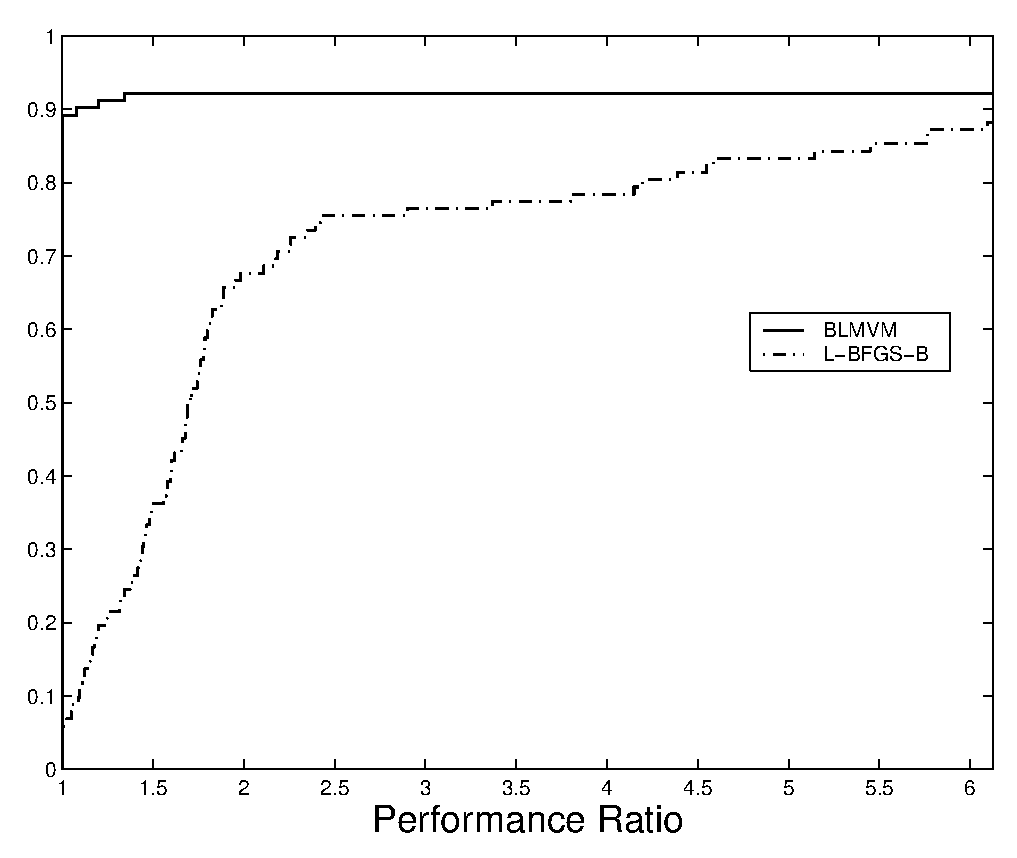
\includegraphics[width=0.45\textwidth,height=0.4\textwidth]{h1.eps}}
   \hskip 0.00\textwidth
   \subfigure[Function Evaluations]{
   \label{PFG}
   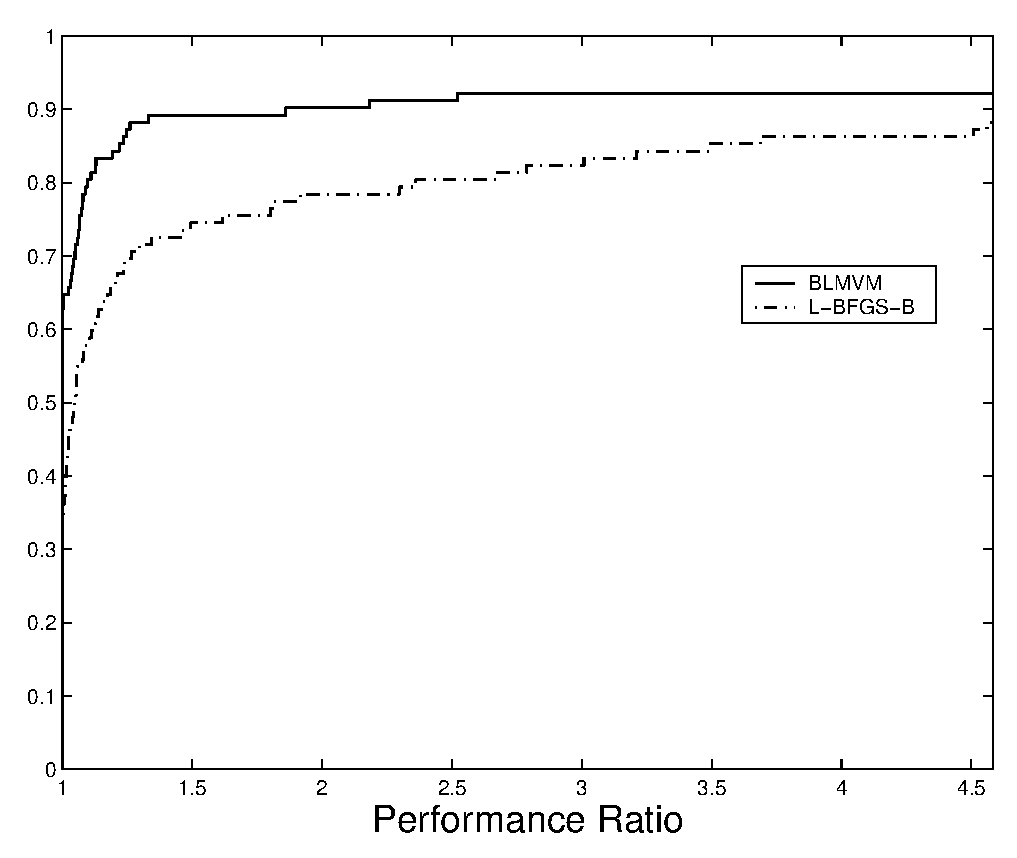
\includegraphics[width=0.45\textwidth,height=0.4\textwidth]{h2.eps}} \\
\label{figure3}
\end{center}
\end{figure}

We applied the performance profiling techniques introduced by Dolan
and Mor\'e\cite{dolan2} to
interpret the results.
Their profiles require a single statistic that measures the performance
of a solver on a problem.  We computed one profile using execution time
and another using the number of function and gradient evaluations.

To create these performance profiles, we first identify the best solver
for each  problem in the test suite.  
Then we compute the ratio of each solver's performance
versus the performance of the best solver.  A ratio of $1.0$ indicates
that the solver was at least as good as the other solvers on that problem
while a ratio greater than one indicates how much worse the solver performed
compared to the best solver.  
When a solver failed to find a solution satisfying the 
specified criteria, we set the ratio to $+\infty$.

Given these ratios, we define a function for each solver.  For every
number greater than or equal to one, this function is
defined to be the percentage of instances where the solver's performance
ratio is less than this number.  This cumulative distribution function
can be plotted for each solver.
The left side of the graph shows how often each solver was the best solver
and the right side of the graph show how often each solver successfully
found a solution.

Figures \ref{figure3} compare the performance of BLMVM to L-BFGS-B
using execution time and number of function evaluations. In both
algorithms, the function and gradient vector were evaluated in
the same routine.
The right side of each graph indicates the robustness of each algorithm
by the percentage of problems that
each algorithm successfully solved.  
Both algorithms fared well by solving about %90/%$ of
the problems to the prescribed accuracy.  BLMVM failed on 8 problems
while L-BFGS-B failed on 12 problems.

The left side of the graphs show the percentage of instances in which each
algorithm performed better than the other.  In terms of function
evaluations, BLMVM used fewer evaluations on about $60\%$ of the problems
while L-BFGS-B used fewer function evaluations on about $30\%$ of the problems.
In terms of execution time, BLMVM performed better on $90\%$ of the test suite,
while  L-BFGS-B used less time on only a few problems.

In addition, we found that when function evaluations were used a measure,
BLMVM performed L-BFGS-B by a factor of two on $15\%$ of the problems and
a factor of three on $10\%$ of the problems.   When execution time was used
as the measure, BLMVM performed L-BFGS-B by a factor of two on $25\%$ of the problems and
a factor of three on $15\%$ of the problems.
On average, BLMVM was about $40\%$ faster than
the competition.  

Since BLMVM uses fewer function evaluations on most problems, we feel that the
step direction used in BLMVM is better than the one used by  L-BFGS-B.  
In terms of execution time, BLMVM shows a
distinct advantage.  In all but a few cases, it found a solution
in less time.  These facts indicate that one iteration of the
BLMVM algorithm is usually cheaper that one iteration of L-BFGS-B.
Whereas L-BFGS-B first identifies a face in the feasible region and
then minimizes over that face, BLMVM always computes a step direction
in the full space.  By not explicitly working in a subspace,
BLMVM saves the time that other algorithms spend identifying it.
These features, and the use of the two-loop recursion instead of the compact
form, make the BLMVM algorithm efficient and relatively simple to implement.

\comment{
The fact that the number of evaluations is less indicates that our
step directions are better.  Even though the theorem only applies
to the when the iterates are on the optimal face, we are gradually
eliminating the effects of the gradient in the free variables.
}


\section{Scalability Using Multiple Processors}

To demonstrate the parallel efficiency of the algorithm,
we solved the obstacle problem from the MINPACK-2 test
suite using 1 - 512 processors.  
This benchmark is a variational problem over a two
dimensional region.  
It asks for the surface with the least area that satisfies a 
set of boundary conditions and lies above an obstacle within
the region. 
Given a two dimensional region ${\cD}$, an obstacle $v_L(x)$ defined on
that region, and boundary conditions $v_D (x)$,
the infinite dimensional version of this problem can be stated as

\[
\min \left \{ f(v) :
v \in H^1, \ v(x) = v_D (x) \ \ \forall  x \in \partial \cD, \ 
                v(x) \ge v_L (x) \ \ \forall  x \in \cD
\right \}
\]
where 
\[
f(v) = \int_{\cD} \sqrt{ 1 + \| \grad v(x) \|^2 } \; dx
\]

%\centerline {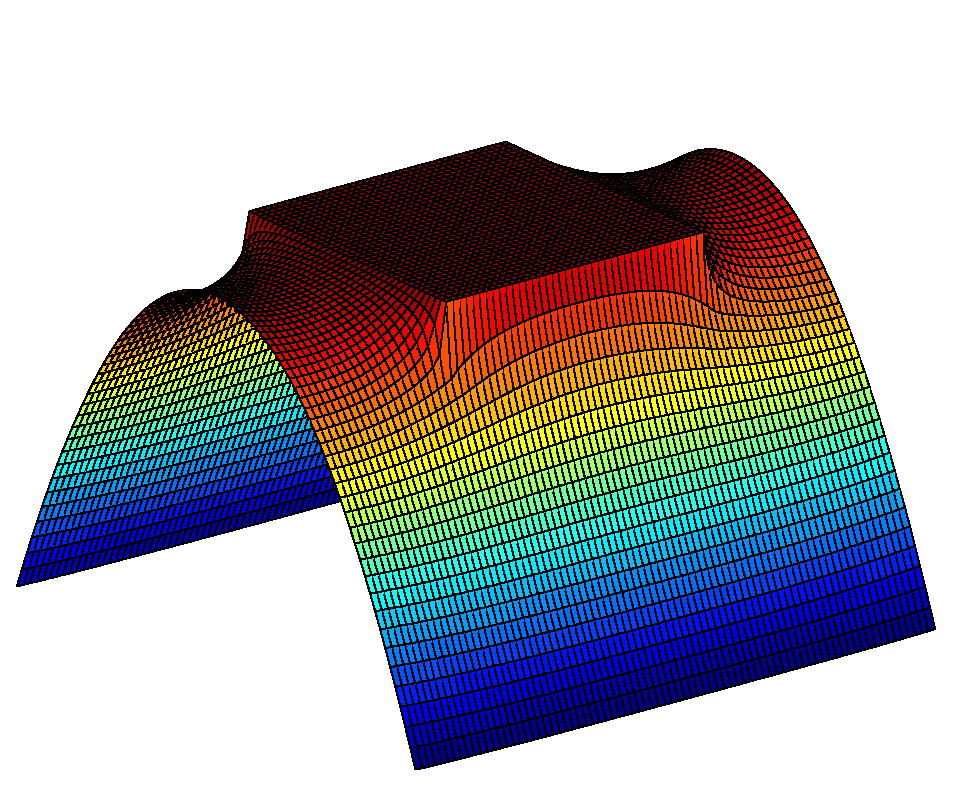
\includegraphics[height=2.1in]{../tutorials/images/mso.eps}}
\centerline {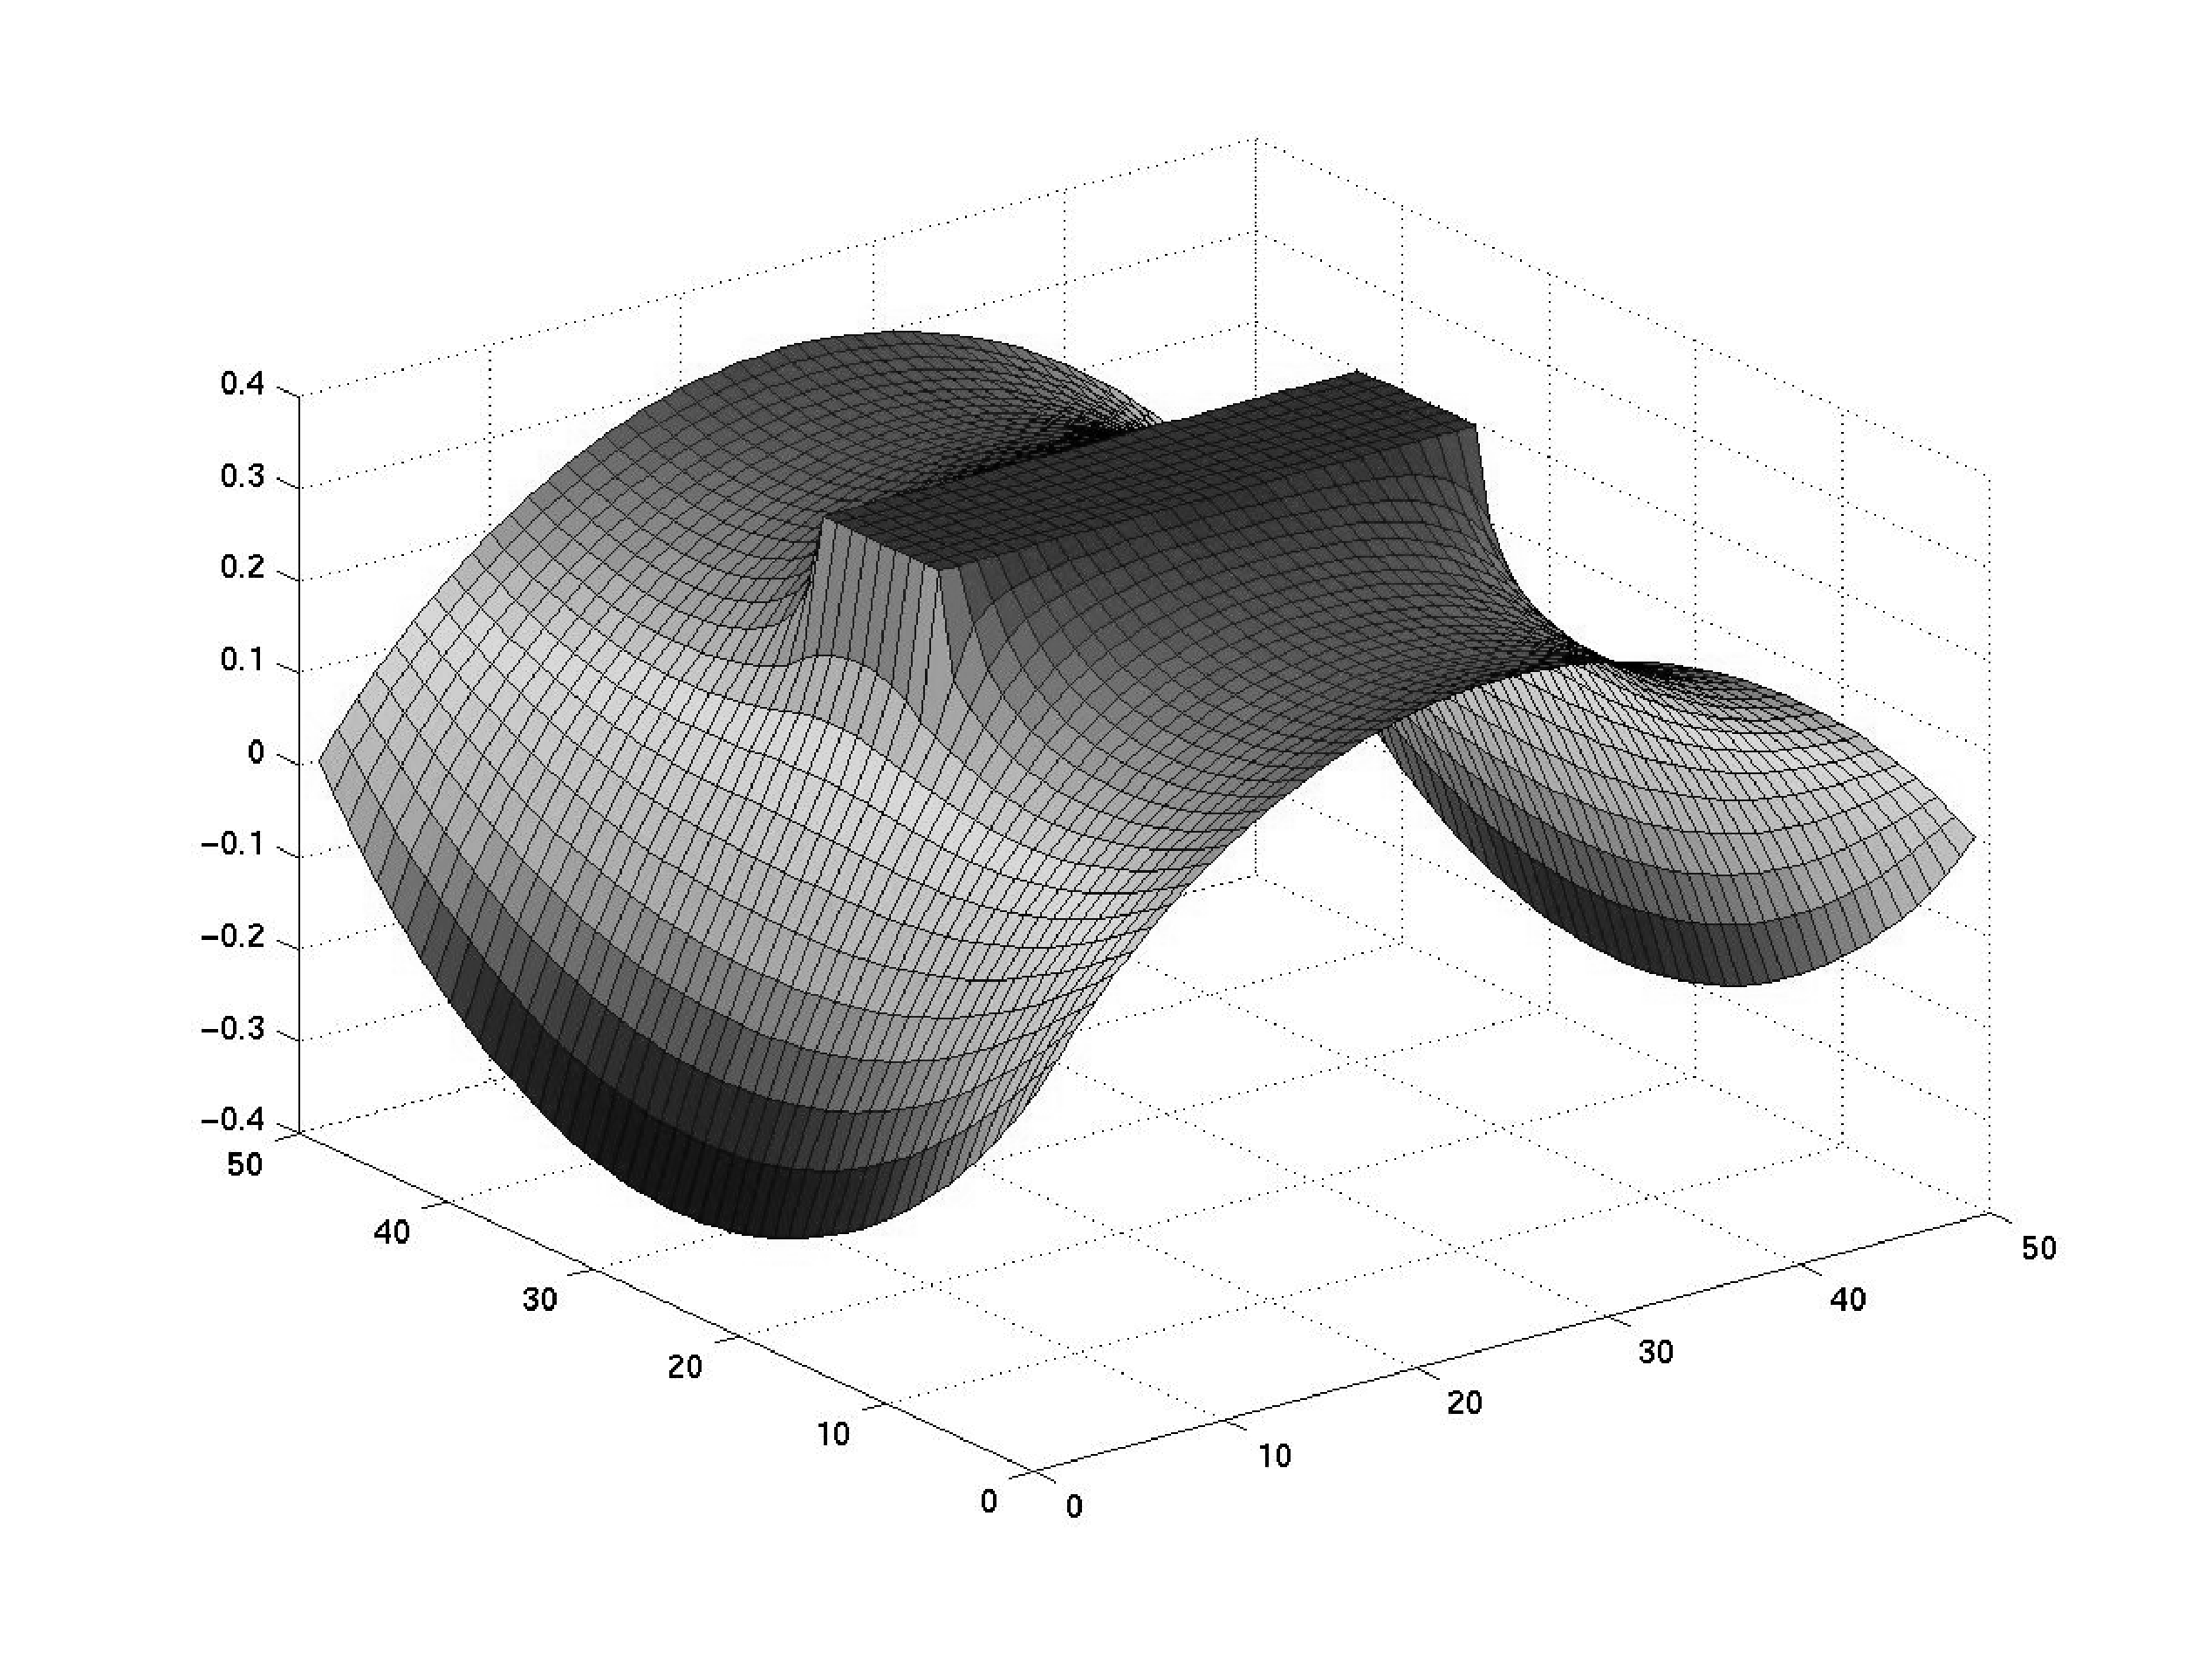
\includegraphics[height=3.1in]{surf5.ps}}

We prepared this problem for parallel computing 
using the grid management facilities of PETSc, 
which relies on MPI \cite{using-mpi} for all
communication between processors.
PETSc provides support for
discretizing the rectangular region ${\cD}$,
partitioning the surface into multiple regions and assigning
each processor to one these regions.  Each processor computes the surface
area of its region and the gradient of the objective value with respect to
the variables in its region.

These computations were performed on the Cray T3E supercomputer at the 
National Energy Research Scientific Computing Center (NERSC).
Each processor on this computer has 256 MB of RAM, and clock speed 
of 450 MHz, and a peak performance of  900 Mflops.  


Our first tests discretized the region into a $1600 \times 1600$ mesh,
which creates $2,560,000$ variables.  The obstacle was a rectangular
plate covered by the $640 \times 960$ mesh points in the middle of the
mesh.  The height of the plate was set to $0.2$.
The memory requirements of a problem
this large are so high that it exhausted the memory of the computer
when only four processors were used.  We solved the problem using as
few as 8 processors and as many as 512 processors.
Table 
\ref{routines} shows the number of iterations,
and seconds used to solve the problem in each test.
The table also indicates the
percentage of time spent in various parts of the algorithm.  The
time spent adding vectors is shown under the label {\tt AXPY}.
This category also includes time spent
copying vectors, projecting vectors, and performing other vector operations 
that do not require communication between processors.  The
{\tt Dot} column indicates the percentage of time spent performing vector
inner products and vector norms.  The column {\tt FG} shows the
percentage of time spent computing the function and gradient.

\begin{table}[bhpt]
\small
\begin{center}
\begin{tabular}{|cccccc|}
\hline
\multicolumn{1}{|c|}{Processors} &
\multicolumn{1}{c|}{BLMVM} &
\multicolumn{1}{c|}{Execution} &
\multicolumn{3}{c|}{Percentage of Time} \\
%\multicolumn{1}{|c|}{} \\
\multicolumn{1}{|c|}{Used}&
\multicolumn{1}{|c|}{Iterations}&
\multicolumn{1}{c|}{Time}&
\multicolumn{1}{c}{AXPY}&
\multicolumn{1}{c}{Dot} &
\multicolumn{1}{c|}{FG} \\
%\multicolumn{1}{c|}{FLOPS} \\

%\hline
%
%1 & 566 & 1226.0 & 29 & 9 & 62 & 36 \\
%2 & 690 & 736.9 & 29 & 9 & 62 & 74 \\
%4 & 559 & 305.9 & 29 & 8 & 63 & 144 \\
%8 & 550 & 172.6 & 26 & 8 & 66 & 251 \\
%16 & 570 &  78.6 & 28 & 11 & 60 & \\
%32 & 691 & 37.6 & & & & \\
%64 & 572 & 21.7 & 24 & 15 & 54 & \\
%128 & 695 & 14.7 & 24 & 20 & 55 & 3725 \\
%256 & 695 & 9.0 & 28 & 27 & 55 & 3725 \\
\hline

8 & 996 & 1083.8 & 31  & 9 & 60 \\ %& 256 \\
16 & 991 & 538.2 & 30 & 10 & 60 \\ %& 580 \\
32 & 966 & 267.7 & 29 & 11 & 60 \\ %& 1137 \\
64 & 993 & 139.5 & 27 & 13 & 60 \\ %& 2027 \\
128 & 987 & 72.4 & 25 & 15 & 60 \\ %& 3728 \\
256 & 996 & 39.2 & 26 & 18 & 56 \\ %& 8009 \\
512 & 1000 & 21.6 & 23 & 22 & 53 \\
\hline
\end{tabular}
\caption{Performance of BLMVM on Obstacle Problem.}
\label{routines}
\end{center}
\end{table}

Since more than $60\%$ of the execution time was spent
evaluating the function and gradient,
an efficient implementation of this routine is mandatory for good 
parallel performance.
Our function has a structure that allows an efficient parallel evaluation,
and its scalability is demonstrated by the fact that the percentage of
time spent in this routine did not increase with the number of processors.

The rest of the time was spent computing the BLMVM step direction and
projecting the new step into the feasible region.  Operations such as
scaling vectors, adding vectors,
copying the elements of one vector to another, and applying the projections 
$P$ and $G$  do not require any communication between processors.
These operations scale very well to more processors, and the percentage
of time spent in these operations declined as the number of processors 
increased.  The bottleneck in numerical computations involve
vector inner products and norms.  
These operations require communication between processors, whose overhead
degrades performance.
In this problem, the percentage of time spent in these operations 
more than doubled from $9\%$ to $22\%$.  

The overall efficiency of our implementation is shown in Figure \ref{G14}.
Each bar indicates the performance of BLMVM of each test relative to
the performance of BLMVM on eight processors.  
This number is the ratio of eight times the execution time using 
eight processors and the number of processors multiplied by the
time need to solve the problem using those processors.
Relative to the performance of BLMVM on this problem using eight processors,
the overall parallel efficiency using 256 processors was over $86\%$
and the overall parallel efficiency using 256 processors was over $78\%$.

In a second set of tests we solved obstacle problem using a mesh that was
refined according the number of processors used to solve the problem.
In these tests each processor owned $10,000$ variables.
The mesh was $100 \times 100$ when one processor was used and 
$1600 \times 1600$ when $256$ processors were used.  The length
and width of the obstacle were adjusted proportionately.  Since BLMVM
uses more iterations to solve problems with  finer meshes, we used
the rate of floating point operations as the measure of efficiency.
Figure \ref{G14chol} shows the average number of floating point operations
performed per second on each processor.  The problem used over $34$ MFlops when
one processor was used and that rate only decreased to about  $31$ MFlops when
when 256 processors were used.
Our parallel efficiency by this measure was over $90\%$.


\begin{figure}[ht]
\begin{center}
\caption{Parallel Efficiency of BLMVM on the Obstacle Problem.}
   \subfigure[Overall Implementation Efficiency]{
   \label{G14}
   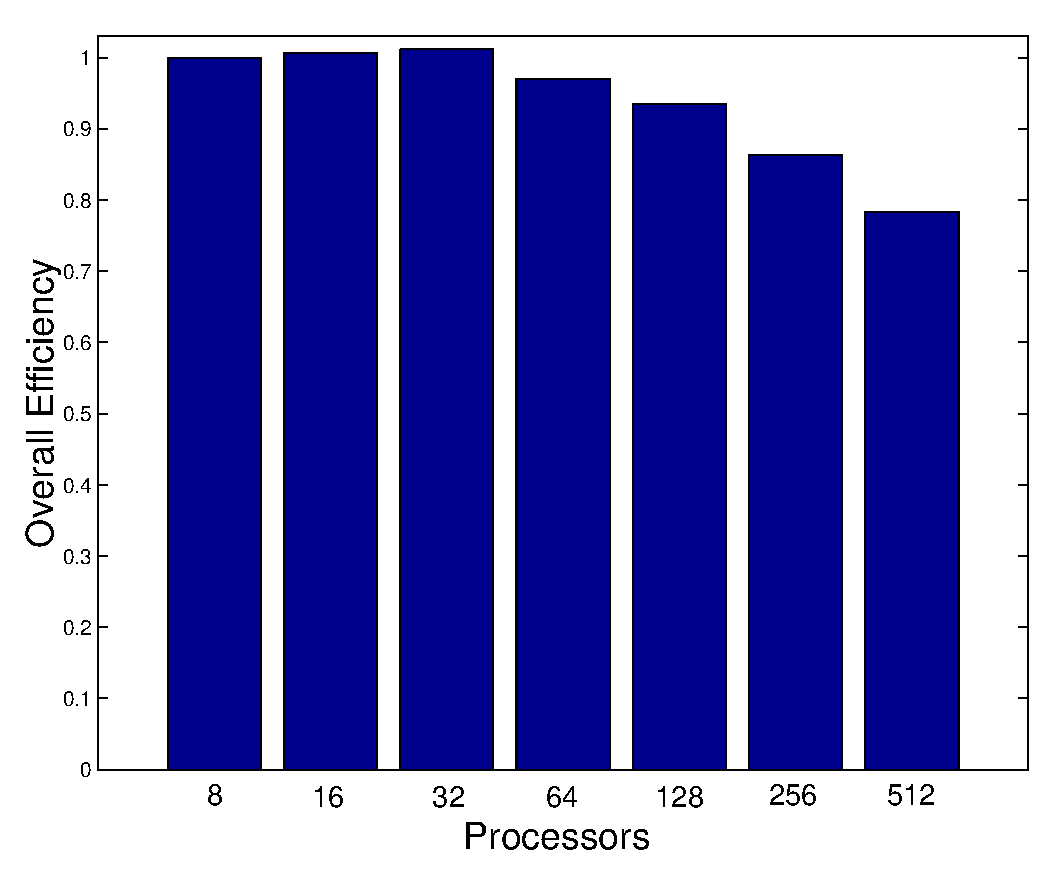
\includegraphics[width=0.45\textwidth,height=0.4\textwidth]{f4.eps}}
   \hskip 0.00\textwidth
   \subfigure[Floating Point Efficiency]{
   \label{G14chol}
   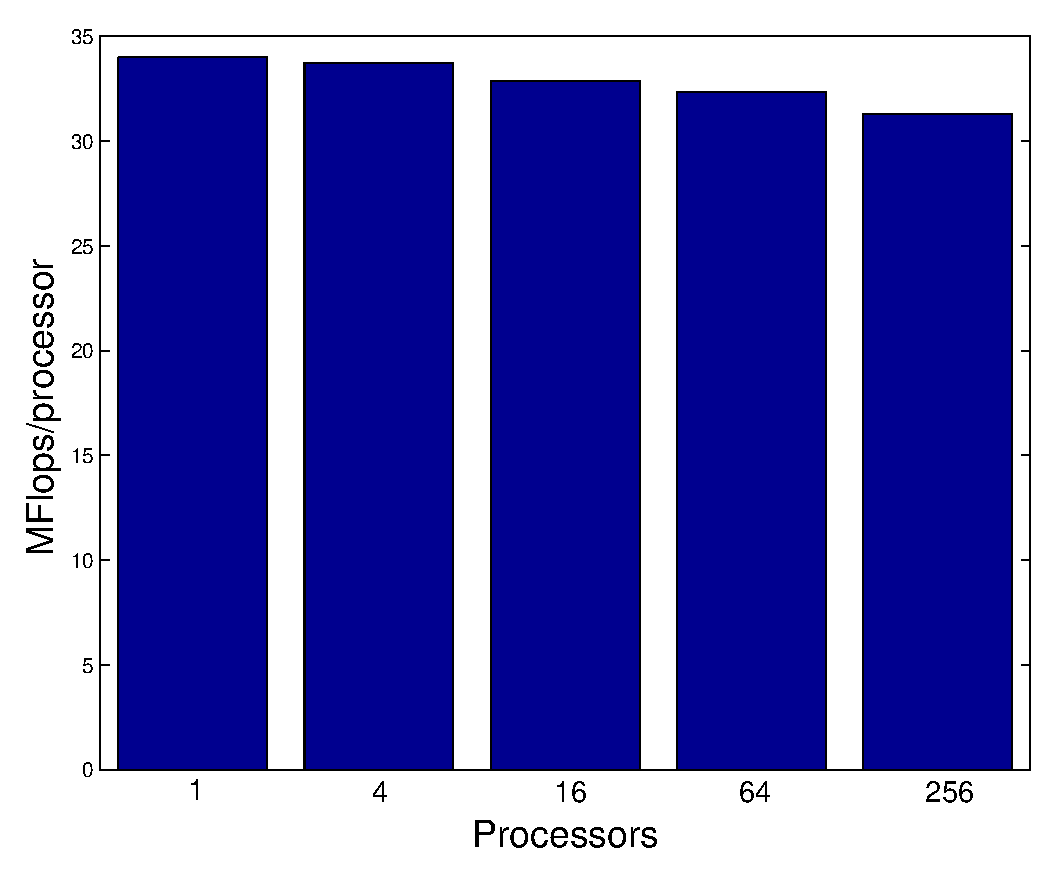
\includegraphics[width=0.45\textwidth,height=0.4\textwidth]{f3.eps}} \\
\label{figure2}
\end{center}
\end{figure}


\section{Conclusion}

We have described a robust and efficient method
bound constrained optimization that requires only 
function and gradient evaluations from the objective function. 
Its limited storage requirements make it well
suited for large optimization problems.  
On some large problems, the algorithm can also compute a
solution in parallel with high level of efficiency.
Against other solvers in its class, numerical experiments showed
that it performed very well.

Our implementation of this algorithm is available in 
the Toolkit for Advanced Optimization (TAO).  
The TAO project \cite{tao-web-page,tao-user-ref}
focuses on the design and implementation of
component-based optimization software for the
solution of large-scale optimization applications.
Its design enables connection to lower-level
support (parallel vectors, sparse matrix data
structures, preconditioners, solvers) provided in toolkits such as
PETSc,
and thus we are able to build on top of these toolkits
instead of having to redevelop code. 
Initial work in TAO
has centered on the development of solvers for 
unconstrained and bound-constrained minimization and
nonlinear least squares.


%\input{cg}

\bibliographystyle{siam}

\bibliography{../tao,%
/home/more/papers/bibs/opt80,%
/home/more/papers/bibs/opt90}%

\end{document}

